



\documentclass[a4paper, 10pt]{article} % For LaTeX2e
\usepackage{amsmath}
\usepackage{amssymb}
\usepackage[colorlinks=true,
            linkcolor=red,
            urlcolor=blue,
            citecolor=gray]{hyperref}
\usepackage[utf8]{inputenc}
\usepackage[T1]{fontenc}
\usepackage{lmodern}
\usepackage[french]{babel}
%\usepackage{times}
\usepackage{graphicx}
\usepackage{color}
\usepackage[usenames,dvipsnames,svgnames,table]{xcolor}
\usepackage{multirow}
\usepackage[authoryear,round]{natbib}
\usepackage{bbm}
\usepackage{latexsym}
\usepackage{epsfig}
\usepackage{subfigure}
\usepackage{placeins}
\usepackage{algorithmic}
\usepackage{algorithm}
\usepackage{rotating}
\usepackage{hyperref}
\usepackage{fancyhdr}
\usepackage{alltt}
\usepackage[left=2cm,right=2cm,top=3cm,bottom=2cm]{geometry}

% TikZ
\usepackage{pgf}
\usepackage{tikz}
\usetikzlibrary{arrows}

% Where can LaTeX find figures ?
\graphicspath{{images/}}

% PDF informations
%-----------------------------------------------------------------
\hypersetup{%
  a4paper=true,
  pdfstartview=FitH,
  colorlinks=true,
  pdfborder=0 0 0,
  pdftitle    = {INC Fall2013 : Spécification du protocole de communication avec le périphérique},
  pdfsubject  = {},
  pdfauthor   = {Xavier Lagorce},
  pdfkeywords = {INC, Fall2013, protocole, communication, clef}}

%\usepackage{vmargin}            % red?finir les marges
%\setmarginsrb{3cm}{3cm}{3cm}{3cm}{1cm}{2cm}{1cm}{2cm}

% Configuration des headers
\pagestyle{fancy}
%\fancyhead{} %Effacer les headers
\lhead{Projet KeyBox}
\rhead{Communication avec le périphérique}

\newcommand{\saut}{\vspace{0.5cm}}
\newcommand{\rien}{-}
\title{{\huge KeyBox}\vspace{0.5cm}\\Spécifications du protocole de communication avec le périphérique}
\author{\href{mailto:Xavier.Lagorce@crans.org}{Xavier Lagorce}\\\href{mailto:laurent.cabaret@ecp.fr}{Laurent Cabaret}}
\date{21 Octobre 2013 - v1.0\\Ce document est sujet à modifications}

\begin{document}

\maketitle

\vspace{1cm}

\tableofcontents
\newpage

\section{Introduction}

Le présent document spécifie le protocole de communication utilisé entre l'hôte (la centrale)
et le périphérique (boîtier de clef dont l'ID est le numéro du groupe (exemple Gr7 $\longrightarrow 07$)).

\section{Medium}

La communication entre l'hôte et le périphérique se fera à travers une liaison propriétaire fournissant un port série (Tx et Rx) \footnote{Cela correspond au type de liaison série utilisée lors de la formation Arduino.} ainsi que 2 alimentations 5V et 12V et une masse.

\saut

\subsection{Liaison série}
La liaison série aura les paramètres suivants\footnote{Ces paramètres sont le plus souvent regroupés
sous l'appellation 9600/8N1} :
\begin{itemize}
  \item vitesse de communication : 9600 bps
  \item 8 bits de données
  \item pas de bit de parité
  \item 1 bit de stop
\end{itemize}

\subsection{Connecteur}

Nous allons utiliser un connecteur à dix contacts 5x2 

\begin{center}
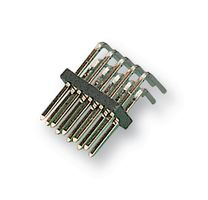
\includegraphics[scale=0.5]{HE10.jpg}
\end{center}

dont le brochage devra obligatoirement être le suivant :

\begin{center}
\begin{tabular}{r|c||c|l}
GND&1&10&Nc\\
5V&2&9&Nc\\
12V&3&8&Nc\\
TxO&4&7&Nc\\
RxI&5&6&Nc\\
\end{tabular}
\end{center}


\begin{itemize}
\item TxO sera connecté au Tx de l'arduino
\item RxI sera connecté au Rx de l'arduino
\end{itemize}


Ce point étant critique, il est obligatoire de contacter le responsable du design de la communication de la centrale\footnote{laurent.cabaret@ecp.fr} avant l'impression  de votre carte prototype.
En effet le sens du connecteur (Top/Bottom/...) du coté centrale n'est pas modifiable.

Nous rappelons que lors de la soutenance il faudra très rapidement pouvoir connecter la centrale a votre système sans démonter de plus de 5s. Tout problème dans cette communication sera considéré comme une erreur de conception.

\section{Protocole}

\subsection{Format des commandes}

Une commande envoyée par l'hôte sera une chaîne de caractères ASCII lisibles par un humain. elle aura la
forme suivante :
\begin{center}
  \verb|IIPPP<cr>|
\end{center}

où :
\begin{itemize}
  \item \verb|II| est à remplacer par les lettres codant une commande particulière
  \item \verb|PPP| est à remplacer par l'éventuel argument associé à la commande (il sera remplacé par '\verb|___|' si
    la commande ne demande pas d'argument).
  \item \verb|<cr>|\footnote{<cr> est un caractère spécial : carriage return ou retour chariot \href{http://fr.wikipedia.org/wiki/American_Standard_Code_for_Information_Interchange}{Code Acsii}}
\end{itemize}

\subsection{Liste des commandes}
\begin{itemize}

  \item \textbf{Donner l'information de présence clef (CP)}
    \begin{center}\verb|CP_ID|\end{center}
    Cette commande demande au périphérique de donner l'information de présence de la clef.
    Le périphérique ne doit répondre à cette commande uniquement si l'ID est celui de la boite.

\saut

  \item \textbf{Libérer la clef (CF)}
    \begin{center}\verb|CF_ID|\end{center}
    Cette commande demande au périphérique de donner l'ordre de libération de la clef.
    Le périphérique ne doit obéir à cette commande uniquement si l'ID est celui de la boite.
\saut 

  \item \textbf{Réponse de la présence clef (KP)}
    \begin{center}\verb|KPVID|\end{center}
	Indique à la centrale la présence ou non de la clef.
	
	\verb|KPYID| : Clef présente.
	
	\verb|KPNID| : Clef absente.
\end{itemize}


\section{Exemple type d'une conversation}
\begin{center}
\begin{tabular}{|c|c|p{6cm}|}
\hline
Centrale&KeyBox&\\
\hline
\hline
\verb|CP_07<cr>|&\rien& La centrale demande : Présence clef ?\\
\rien&\verb|KPY07<cr>|& La KeyBox répond : Oui\\
\hline
\vdots&\vdots& 	\\
\hline
\verb|CP_07<cr>|&\rien& La centrale demande : Présence clef ?\\
\rien&\verb|KPY07<cr>|& La KeyBox répond : Oui\\
\hline
\verb|CF_07<cr>|&\rien& Ordre de libération de la clef\\
\hline
\verb|CP_07<cr>|&\rien& La centrale demande : Présence clef ?\\
\rien&\verb|KPY07<cr>|& La KeyBox répond : Oui\\
\hline
\verb|CP_07<cr>|&\rien& La centrale demande : Présence clef ?\\
\rien&\verb|KPN07<cr>|&La KeyBox répond : Non\\
\hline
\vdots&\vdots&\\
\hline
\verb|CP_07<cr>|&\rien& La centrale demande : Présence clef ?\\
\rien&\verb|KPY07<cr>|& La KeyBox répond : Oui\\
\hline
\end{tabular}
\end{center}


\end{document}

